\documentclass[10pt]{article}
\usepackage[T1]{fontenc}
\usepackage{lmodern,amsmath,amssymb,graphicx,hyperref}
\usepackage[margin=.74in]{geometry}
\setlength{\parindent}{0pt}\setlength{\parskip}{6pt}
\begin{document}
\begin{center}{\Large An actual anchored interpolation auxiliary}\\[4pt]
17 November2026 --- local unsigned Lean evidence\end{center}
\textbf{Construction.} Over any field $K$, take a public target $(x_t,y_t)$
and three public coordinate pairs $(x_i,y_i)$. The seven interpolation
positions are the target and $(x_i,\pm y_i)$ for $i=0,1,2$.
Require all mixed Taylor coefficients of total degree less than four
to vanish at each position: full ambient multiplicities,
without factorial division [pcc:unverified].

The actual coefficient space and embedding are
\[
 \mathcal C=\{(j,i):0\le j<8,\ 0\le i<16,\ i+2j<16\},\qquad
 E(v)=\sum_{(j,i)\in\mathcal C}v_{j,i}X^iY^j.
\]
Masked nested \texttt{ofFn} linear maps construct $E$.
Each actual double coefficient recovers $v_{j,i}$, so $E$ is injective.
Its image satisfies the previous exact strict budget at
$a=2$, $\ell=7$, $r=4$:
\[
 \deg_Y E(v)\le7,\qquad \deg_X E(v)_j+2j<16.
\]
Zero coefficients have degree $\bot$ [pcc:unverified].

\textbf{Actual operator.}
Taylor translation, coefficient extraction and polynomial linear sums
construct the map $J$ to all seven sets of mixed jets.
There are ten conditions $t+k<4$ per position, hence
\[
 F=J\circ E:K^{72}\longrightarrow K^{70}.
\]
Existing finite-dimension laws show $F$ is not injective.
Kernel laws supply $v\ne0$ with $Fv=0$; injectivity gives $Q=E(v)\ne0$.
The semantic equivalence identifies $Fv=0$ with exactly the specified
multiplicities. No successful signs or kernel vector are supplied as input
[pcc:unverified].

\textbf{Proof map.} The operator's \texttt{anchored\_zero\_iff} binds constraints.

The embedding namespace is \texttt{OrientationAnchoredEmbedding}.
Its ten endpoints include:
\begin{quote}\small
\texttt{coefficientEmbedding\_coordinate}\\
\texttt{coefficientEmbedding\_injective}\\
\texttt{coefficientEmbedding\_budget}\\
\texttt{finiteOperator\_nonzero\_kernel}\\
\texttt{public\_positive\_auxiliary}
\end{quote}
Source019, build020 and receipt010 bind61 statements:51 parent and10 new;
PCC-20261117-51fcf9. Source016, build017 and receipt009 supply10 earlier
operator/index endpoints; PCC-20261117-bdf983 [pcc:unverified].

\textbf{Scope.}
Accepted outputs exit0 without warnings; every printed dependency is among
\texttt{propext}, \texttt{Classical.choice}, \texttt{Quot.sound}.
Local unsigned records are outside shared Transport53/57 audit/fresh.
Classical kernel existence is not an extracted solver.
Four support positions are a fixed control, not a growing family.
Arbitrary coordinates are allowed: curve validity, distinct abscissas and
nonzero ordinates are not inferred. Nonzero polynomial is not yet
nonzero information modulo the curve equation.
\newpage
\begin{center}{\Large Separating the auxiliary from the known curve}\end{center}
\textbf{Actual filter.} For explicit $f\in K[X]$, define
\[
 C_f(Y)=Y^2-f(X),\qquad R_f(Q)=Q\bmod_{\rm monic}C_f.
\]
The actual $C_f$ is monic and nonzero. Existing division laws give
$R_f(Q)=0\Longleftrightarrow C_f\mid Q$.
At every point $y^2=f(x)$, evaluation gives $R_f(Q)(x,y)=Q(x,y)$.

Six checked \texttt{OrientationCurveFilter} endpoints are in
source020, build021 and receipt011:67 statements,61 parent and6 new;
PCC-20261117-fcd5f4. They do not assert nonzero remainder of the generated
auxiliary or preservation of full ambient multiplicities [pcc:unverified].
\begin{center}
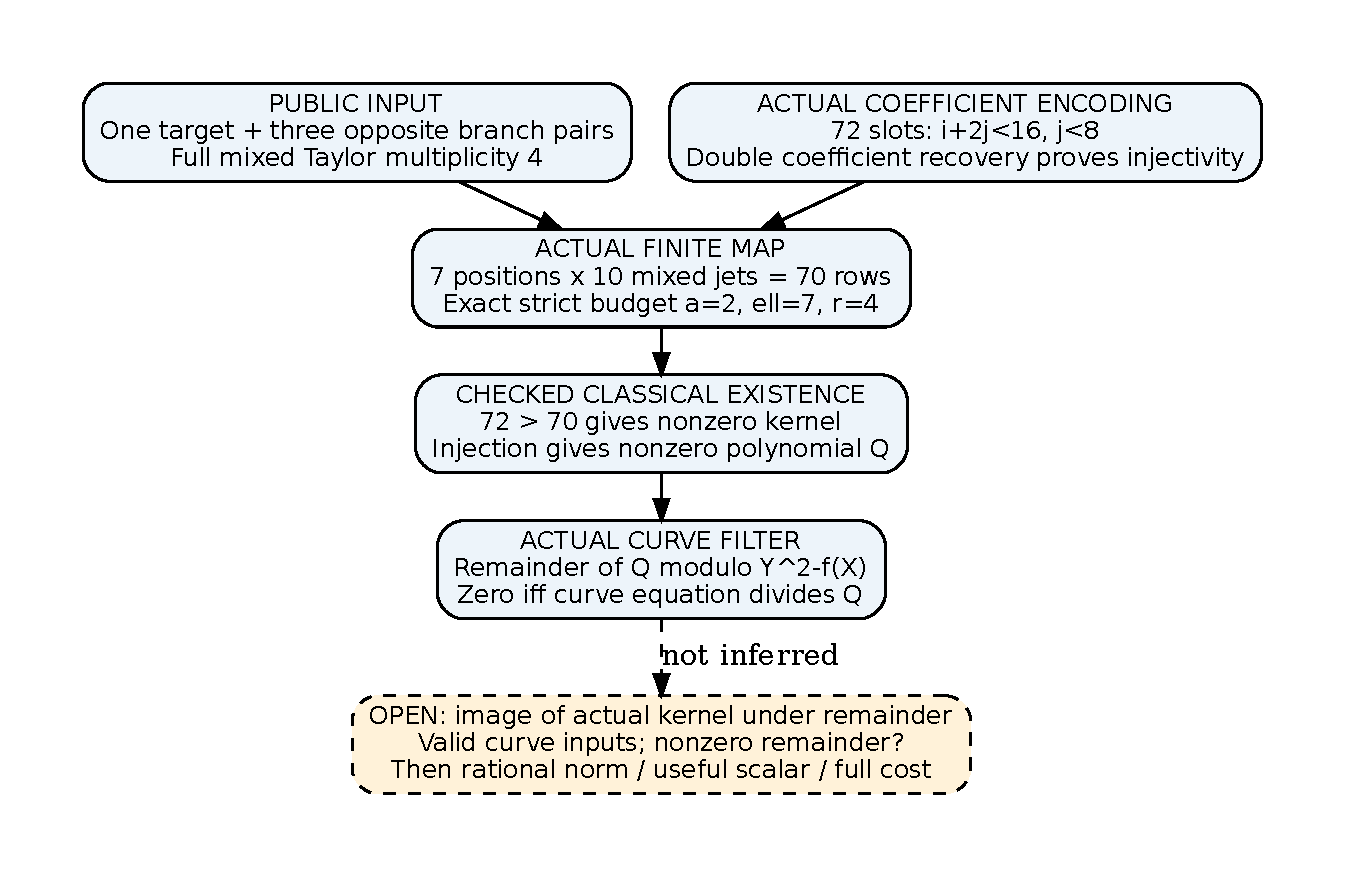
\includegraphics[width=.86\linewidth,height=3.45in,keepaspectratio]{operator-dependencies-001.pdf}
\end{center}
\textbf{Next discriminating obligation.}
Restrict the actual remainder map to the actual finite kernel, under
explicit valid prime-field curve inputs. Establish whether its image has
a nonzero element, with exact parameter scope. Prove any rank/image
compatibility used. Then bind rational substitution, norm/factor extraction,
useful scalar relations and all preparation, field, bit and retry costs.
See versioned \texttt{PROTOCOL-003.md} and continuation013.

\textbf{Reproduction and preservation.}
Instance maps009--011 and exclusive pre-calls pin inputs;
Lean4.35.0 uses default limits. Failed015/017/018 sources and
builds016/018/019 remain. No trust/linter override, native attack,
paid job, timing/scaling campaign or old proof replay.
The frozen uniform report is historical; this diagram is the current
construction. No speed dashboard change is warranted.
Protected remote PCC history remains unresolved; no push/history rewrite.

\textbf{Sources.}
\href{https://doi.org/10.1109/TIT.2013.2243800}{Beelen et al (2013), SectionIII/Theorem6/(2)};
read scope in literature-review001. Mathlib OfFn, Taylor, Div, Monic,
Dimension Constructions and Submodule Ker laws are reused as stated.
KB unavailable; no novelty claim for these methods.
\end{document}
